\chapter{Relative Motion and Kinematics in Moving Frames}
\label{ch:relative}

\begin{chapterintro}
\textbf{Chapter Objectives:} All motion in physics is relative to an observer's frame of reference. In this chapter, you will master the operator relation connecting time derivatives between fixed and rotating frames; prove the classical laws of velocity and acceleration composition; and unveil the kinematic origin of the Coriolis acceleration $2\vec{\Omega}\times\vec{v}_r$.
\end{chapterintro}

\section{Reference Frames and the Moving Basis}

Let $\mathcal{R}(O, \ihat, \jhat, \khat)$ be a reference frame assumed fixed (inertial), and let $\mathcal{R}'(O', \ihat', \jhat', \khat')$ be a secondary reference frame moving with respect to $\mathcal{R}$.
The motion of $\mathcal{R}'$ relative to $\mathcal{R}$ is completely specified by:
\begin{enumerate}[leftmargin=1.5em,itemsep=2pt]
  \item The translational position and velocity of its origin: $\vec{OO'}(t)$ and $\vec{v}_{\mathcal{R}}(O') = \left(\frac{\dd\vec{OO'}}{\dd t}\right)_{\mathcal{R}}$.
  \item Its instantaneous \textbf{angular velocity vector} $\vec{\Omega}_{\mathcal{R}'/\mathcal{R}}(t)$ characterizing the rotation of its basis vectors $(\ihat', \jhat', \khat')$.
\end{enumerate}

\begin{figure}[htbp]
\centering
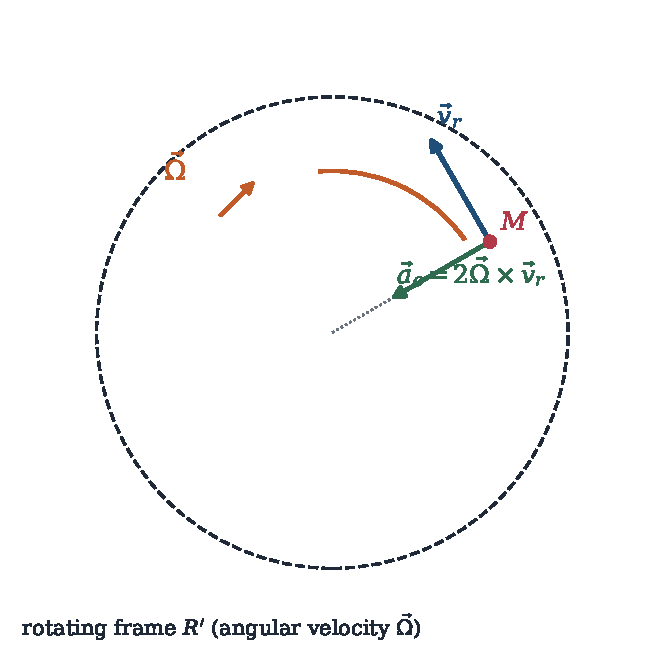
\includegraphics[width=0.74\textwidth]{figures/10_rotating_frame.pdf}
\caption{A particle $M$ observed from both a fixed frame $\mathcal{R}$ and a moving rotating frame $\mathcal{R}'$ with angular velocity $\vec{\Omega}$.}
\label{fig:relative_frame}
\end{figure}

\begin{historicalbox}{Gaspard-Gustave de Coriolis (1792--1843)}
\begin{minipage}{0.28\textwidth}
\centering
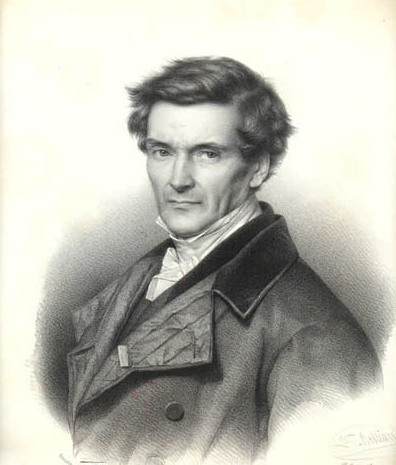
\includegraphics[width=0.95\textwidth]{images/coriolis.jpg}
\captionof{figure}{Gaspard-Gustave de Coriolis (1792--1843), French mathematician and mechanical engineer.}
\end{minipage}\hfill
\begin{minipage}{0.68\textwidth}
Trained at the École Polytechnique, Coriolis was investigating the efficiency of waterwheels, rotating turbines, and mechanical engines with spinning components when he published his landmark 1835 paper \emph{``Sur les équations du mouvement relatif des systèmes de corps''}.

Coriolis demonstrated mathematically that an observer located on a rotating platform detects a subtle supplementary acceleration $2\vec{\Omega}\times\vec{v}_r$ acting on any moving object. Though originally derived for industrial machinery, the Coriolis acceleration became the key to understanding global meteorology, trade winds, cyclonic storms, and oceanic currents.
\end{minipage}
\end{historicalbox}

\section{The Fundamental Kinematic Derivative Operator}

Let $\vec{A}(t) = A_x'\ihat' + A_y'\jhat' + A_z'\khat'$ be an arbitrary vector.
Its time derivative as evaluated by an observer stationary in $\mathcal{R}'$ is:
\[
\left(\frac{\dd\vec{A}}{\dd t}\right)_{\mathcal{R}'} \equiv \dot{A}_x'\ihat' + \dot{A}_y'\jhat' + \dot{A}_z'\khat'.
\]
However, for an observer in $\mathcal{R}$, the basis vectors $(\ihat', \jhat', \khat')$ also rotate according to Poisson's relation $\dot{\vec{u}}' = \vec{\Omega}\times\vec{u}'$:
\[
\left(\frac{\dd\vec{A}}{\dd t}\right)_{\mathcal{R}} = \left(\dot{A}_x'\ihat' + \dot{A}_y'\jhat' + \dot{A}_z'\khat'\right) + \left(A_x'\frac{\dd\ihat'}{\dd t} + A_y'\frac{\dd\jhat'}{\dd t} + A_z'\frac{\dd\khat'}{\dd t}\right).
\]
Substituting $\frac{\dd\vec{u}'}{\dd t} = \vec{\Omega}\times\vec{u}'$:
\[
A_x'(\vec{\Omega}\times\ihat') + A_y'(\vec{\Omega}\times\jhat') + A_z'(\vec{\Omega}\times\khat') = \vec{\Omega}\times\left(A_x'\ihat' + A_y'\jhat' + A_z'\khat'\right) = \vec{\Omega}\times\vec{A}.
\]
We arrive at the fundamental operator identity:
\[
\boxed{\left(\frac{\dd\vec{A}}{\dd t}\right)_{\mathcal{R}} = \left(\frac{\dd\vec{A}}{\dd t}\right)_{\mathcal{R}'} + \vec{\Omega}\times\vec{A}.}
\]

\section{Composition of Velocities}

The absolute position of a particle $M$ is $\vec{r} = \vec{OM} = \vec{OO'} + \vec{r}'$, where $\vec{r}' = \vec{O'M}$.
Differentiating with respect to time in frame $\mathcal{R}$:
\[
\vec{v}_a \equiv \left(\frac{\dd\vec{OM}}{\dd t}\right)_{\mathcal{R}} = \left(\frac{\dd\vec{OO'}}{\dd t}\right)_{\mathcal{R}} + \left(\frac{\dd\vec{r}'}{\dd t}\right)_{\mathcal{R}}.
\]
Applying the operator identity to $\vec{r}'$:
\[
\left(\frac{\dd\vec{r}'}{\dd t}\right)_{\mathcal{R}} = \left(\frac{\dd\vec{r}'}{\dd t}\right)_{\mathcal{R}'} + \vec{\Omega}\times\vec{r}' = \vec{v}_r + \vec{\Omega}\times\vec{r}'.
\]
Therefore:
\[
\boxed{\vec{v}_a = \vec{v}_r + \vec{v}_e,}
\]
where:
\begin{itemize}[leftmargin=1.4em,itemsep=3pt]
  \item $\vec{v}_a = \left(\frac{\dd\vec{OM}}{\dd t}\right)_{\mathcal{R}}$ is the \textbf{absolute velocity} (observed in fixed frame $\mathcal{R}$);
  \item $\vec{v}_r = \left(\frac{\dd\vec{O'M}}{\dd t}\right)_{\mathcal{R}'}$ is the \textbf{relative velocity} (observed in moving frame $\mathcal{R}'$);
  \item $\vec{v}_e = \vec{v}(O') + \vec{\Omega}\times\vec{r}'$ is the \textbf{velocity of transport} (\emph{vitesse d'entraînement}), representing the velocity in $\mathcal{R}$ of the geometric point of $\mathcal{R}'$ coincident with $M$ at that instant.
\end{itemize}

\section{Composition of Accelerations and the Coriolis Term}

Differentiating the absolute velocity $\vec{v}_a = \vec{v}_r + \vec{v}(O') + \vec{\Omega}\times\vec{r}'$ in frame $\mathcal{R}$:
\begin{align*}
\vec{a}_a &= \left(\frac{\dd\vec{v}_a}{\dd t}\right)_{\mathcal{R}} = \left(\frac{\dd\vec{v}_r}{\dd t}\right)_{\mathcal{R}} + \left(\frac{\dd\vec{v}(O')}{\dd t}\right)_{\mathcal{R}} + \left(\frac{\dd\vec{\Omega}}{\dd t}\right)_{\mathcal{R}}\times\vec{r}' + \vec{\Omega}\times\left(\frac{\dd\vec{r}'}{\dd t}\right)_{\mathcal{R}} \\
&= \left[\left(\frac{\dd\vec{v}_r}{\dd t}\right)_{\mathcal{R}'} + \vec{\Omega}\times\vec{v}_r\right] + \vec{a}(O') + \dot{\vec{\Omega}}\times\vec{r}' + \vec{\Omega}\times\left[\vec{v}_r + \vec{\Omega}\times\vec{r}'\right].
\end{align*}
Combining terms:
\[
\boxed{\vec{a}_a = \vec{a}_r + \vec{a}_e + \vec{a}_c,}
\]
where:
\begin{align}
\vec{a}_r &= \left(\frac{\dd^2\vec{r}'}{\dd t^2}\right)_{\mathcal{R}'} \quad \text{(\textbf{Relative Acceleration})}, \\
\vec{a}_e &= \vec{a}(O') + \dot{\vec{\Omega}}\times\vec{r}' + \vec{\Omega}\times(\vec{\Omega}\times\vec{r}') \quad \text{(\textbf{Transport Acceleration})}, \\
\vec{a}_c &= 2\,\vec{\Omega}\times\vec{v}_r \quad \text{(\textbf{Coriolis Acceleration})}.
\end{align}

\begin{lawbox}{Properties of the Coriolis Acceleration $\vec{a}_c = 2\vec{\Omega}\times\vec{v}_r$}
\begin{enumerate}[leftmargin=1.5em,itemsep=2pt]
  \item \textbf{Kinematic Origin}: $\vec{a}_c$ arises from two distinct physical sources of equal magnitude $\vec{\Omega}\times\vec{v}_r$:
  \begin{itemize}[leftmargin=1.2em]
    \item The rotation of the relative velocity vector $\vec{v}_r$ as seen from $\mathcal{R}$: $\vec{\Omega}\times\vec{v}_r$.
    \item The change in transport velocity $\vec{\Omega}\times\vec{r}'$ as the particle moves to a new position $\dd\vec{r}' = \vec{v}_r\dd t$: $\vec{\Omega}\times\vec{v}_r$.
  \end{itemize}
  \item \textbf{Velocity Dependency}: If the particle is stationary in the relative frame ($\vec{v}_r = \vzero$), the Coriolis acceleration is identically zero ($\vec{a}_c = \vzero$).
  \item \textbf{Orthogonality}: $\vec{a}_c$ is always perpendicular to the relative velocity ($\vec{a}_c\cdot\vec{v}_r = 0$) and perpendicular to the rotation axis ($\vec{a}_c\cdot\vec{\Omega} = 0$).
\end{enumerate}
\end{lawbox}

\section{Extensive Worked Examples}

\begin{workedexample}{Bug Crawling Radially on a Rotating Turntable}
A horizontal turntable rotates about its central vertical axis at constant angular velocity $\vec{\Omega} = \omega\khat$.
A beetle crawls along a straight radial line painted on the turntable at constant relative speed $u$ outward from the center: $r'(t) = ut$.
(a) Determine the relative velocity $\vec{v}_r$ and relative acceleration $\vec{a}_r$.
(b) Determine the velocity of transport $\vec{v}_e$ and acceleration of transport $\vec{a}_e$.
(c) Determine the Coriolis acceleration $\vec{a}_c$.
(d) Calculate the absolute acceleration $\vec{a}_a$ and verify by differentiating the absolute position in polar coordinates.

\paragraph{Solution.}

(a) In the rotating frame $\mathcal{R}'(O, \ur, \ut, \khat)$ attached to the turntable:
\[
\vec{r}'(t) = ut\,\ur.
\]
The relative velocity is:
\[
\vec{v}_r = \left(\frac{\dd\vec{r}'}{\dd t}\right)_{\mathcal{R}'} = \dot{r}'\ur = \boxed{u\,\ur.}
\]
Since $u = \text{const}$, the relative acceleration is:
\[
\vec{a}_r = \left(\frac{\dd\vec{v}_r}{\dd t}\right)_{\mathcal{R}'} = \boxed{\vzero.}
\]

(b) For transport kinematics (with $O'=O \implies \vec{a}(O')=\vzero$, and $\dot{\vec{\Omega}}=\vzero$):
\[
\vec{v}_e = \vec{\Omega}\times\vec{r}' = (\omega\khat)\times(ut\,\ur) = \omega ut(\khat\times\ur) = \boxed{\omega ut\,\ut.}
\]
The transport acceleration is the centripetal acceleration of the turntable surface:
\[
\vec{a}_e = \vec{\Omega}\times(\vec{\Omega}\times\vec{r}') = (\omega\khat)\times(\omega ut\,\ut) = \omega^2 ut(\khat\times\ut) = \boxed{-\omega^2 ut\,\ur.}
\]

(c) The Coriolis acceleration is:
\[
\vec{a}_c = 2\,\vec{\Omega}\times\vec{v}_r = 2(\omega\khat)\times(u\,\ur) = 2\omega u(\khat\times\ur) = \boxed{2\omega u\,\ut.}
\]
Notice that $\vec{a}_c$ points forward along the tangential direction of rotation!

(d) The total absolute acceleration is the vector sum:
\[
\vec{a}_a = \vec{a}_r + \vec{a}_e + \vec{a}_c = \vzero - \omega^2 ut\,\ur + 2\omega u\,\ut = \boxed{-\omega^2 r\,\ur + 2\omega u\,\ut.}
\]
\textbf{Verification via polar coordinates in fixed frame $\mathcal{R}$:}
The particle has polar coordinates $r(t) = ut$, $\theta(t) = \omega t$.
Thus $\dot{r} = u, \ddot{r} = 0, \dot{\theta} = \omega, \ddot{\theta} = 0$.
The polar acceleration formula gives:
\begin{align*}
a_r &= \ddot{r} - r\dot{\theta}^2 = 0 - (ut)\omega^2 = -\omega^2 r, \\
a_\theta &= r\ddot{\theta} + 2\dot{r}\dot{\theta} = r(0) + 2(u)(\omega) = 2\omega u.
\end{align*}
Thus $\vec{a}_a = -\omega^2 r\,\ur + 2\omega u\,\ut$, matching the composition of accelerations theorem identically!
\end{workedexample}

\begin{workedexample}{Apparent Wind on a Fast Racing Sailboat}
A racing catamaran sails due North at a speed of $v_b = 20.0\ \mathrm{knots} \approx 10.3\ \mathrm{m\,s^{-1}}$ relative to the water.
A true atmospheric wind blows from the West at $v_w = 12.0\ \mathrm{knots} \approx 6.17\ \mathrm{m\,s^{-1}}$ (pointing due East).
(a) Determine the magnitude and direction of the \textbf{apparent wind} $\vec{v}_{\text{app}}$ experienced by the sailors aboard the catamaran.
(b) If the boat accelerates to $v_b = 30.0\ \mathrm{knots}$, calculate the new apparent wind speed and angle.

\paragraph{Solution.}

(a) Set up Cartesian coordinates with $\ihat$ pointing East and $\jhat$ pointing North.
The velocity of the boat relative to the water (moving frame $\mathcal{R}'$) is:
\[
\vec{v}_b = v_b\,\jhat = 20.0\,\jhat\ \mathrm{knots}.
\]
The true wind velocity relative to the water (fixed frame $\mathcal{R}$) is:
\[
\vec{v}_{\text{true}} = v_w\,\ihat = 12.0\,\ihat\ \mathrm{knots}.
\]
By the velocity addition theorem, $\vec{v}_{\text{true}} = \vec{v}_{\text{app}} + \vec{v}_b$.
Therefore, the apparent wind observed aboard the boat is:
\[
\vec{v}_{\text{app}} = \vec{v}_{\text{true}} - \vec{v}_b = 12.0\,\ihat - 20.0\,\jhat\ \mathrm{knots}.
\]
Magnitude:
\[
v_{\text{app}} = \sqrt{(12.0)^2 + (-20.0)^2} = \sqrt{144 + 400} = \sqrt{544} \approx \mathbf{23.3\ \mathrm{knots}} \approx 12.0\ \mathrm{m\,s^{-1}}.
\]
Direction angle $\theta$ measured from the bow (North, $-\jhat$ direction):
\[
\tan\theta = \frac{v_{\text{app}, x}}{\abs{v_{\text{app}, y}}} = \frac{12.0}{20.0} = 0.600 \implies \theta = \arctan(0.600) \approx \mathbf{31.0^\circ.}
\]
The sailors feel a strong $23.3\ \mathrm{knot}$ wind coming from $31^\circ$ off the starboard bow!

(b) When boat speed increases to $v_b = 30.0\ \mathrm{knots}$:
\[
\vec{v}_{\text{app}} = 12.0\,\ihat - 30.0\,\jhat\ \mathrm{knots}.
\]
\[
v_{\text{app}} = \sqrt{12.0^2 + 30.0^2} = \sqrt{144 + 900} = \sqrt{1044} \approx \mathbf{32.3\ \mathrm{knots}}.
\]
Angle:
\[
\tan\theta = \frac{12.0}{30.0} = 0.400 \implies \theta = \arctan(0.400) \approx \mathbf{21.8^\circ.}
\]
As the boat accelerates, the apparent wind shifts closer to the bow (the wind ``comes forward''), requiring the crew to sheet the sails in tightly like an aircraft wing.
\end{workedexample}
